\documentclass{beamer}

\mode<presentation>{
	%\usetheme{CambridgeUS}
	%\usecolortheme{seahorse}
	\usetheme{Boadilla}
	\usecolortheme{beaver}
	\setbeamertemplate{navigation symbols}{}
}

\usepackage{graphicx}
\usepackage{booktabs}
\usepackage{algpseudocode}
\usepackage{hyperref}
\usepackage{tikz}
\usepackage[utf8]{inputenc}
\usepackage{listings}
\usepackage[export]{adjustbox}
\usepackage{aeguill}

%\setbeamertemplate{title page}[default][rounded=false]

\setbeamertemplate{title page}
{
%\vbox{}
\begingroup
\centering
\begin{beamercolorbox}[sep=8pt,center]{institute}
\usebeamerfont{institute}\insertinstitute
\end{beamercolorbox}
\vskip1em%
\begin{beamercolorbox}[sep=8pt,center]{title}
\usebeamerfont{title}\inserttitle\par%
\ifx\insertsubtitle\@empty%
\else%
\vskip0.25em%
{\usebeamerfont{subtitle}\usebeamercolor[fg]{subtitle}\insertsubtitle\par}%
\fi%
\end{beamercolorbox}%
\vfill
\begin{beamercolorbox}[sep=8pt,center]{author}
\usebeamerfont{author}\insertauthor
\end{beamercolorbox}
\vskip1em\par
\begin{beamercolorbox}[sep=8pt,center]{date}
\usebeamerfont{date}\insertdate
\end{beamercolorbox}
\endgroup
}

\setbeamertemplate{blocks}[default]
\setbeamercolor{structure}{fg=darkred}
%\setbeamercolor{block title}{bg=darkred,fg=white}
%\setbeamercolor{block body}{bg=darkgray!20!white}
\setbeamercolor{block title}{bg=darkgray!30!white}
\setbeamertemplate{enumerate items}[default]

\setbeamertemplate{part page}{
\begin{beamercolorbox}[sep=8pt,center,wd=\textwidth]{part title}
\usebeamerfont{part title}\insertpart\par
\end{beamercolorbox}
\vfill
\tableofcontents
}

%\setbeamertemplate{frametitle continuation}{(\insertcontinuationcount)}

\setbeamertemplate{headline}{\leavevmode\hbox{\begin{beamercolorbox}[wd=.5\paperwidth,ht=2.65ex,dp=1.5ex,center]{section in head/foot}\usebeamerfont{section in head/foot}\insertsectionhead\hspace*{2ex}
\end{beamercolorbox}\begin{beamercolorbox}[wd=.5\paperwidth,ht=2.65ex,dp=1.5ex,center]{subsection in head/foot}\usebeamerfont{subsection in head/foot}\hspace*{2ex}\insertsubsectionhead\end{beamercolorbox}}\vskip0pt}

\setbeamertemplate{background}{\tikz[overlay,remember picture]\node[opacity=0.08]at (current page.south east){
\includegraphics[width=10cm]{figures/unibo_logo.jpg}};}

\newcommand{\tcc}[1]{\textcolor{darkred}{#1}}

\newcommand{\codeA}[1]{\texttt{#1}}
\newcommand{\codeB}[1]{\texttt{\textcolor{darkred}{#1}}}

\newcommand{\link}[1]{{\footnotesize » \url{#1}}}
\newcommand{\bothquote}[1]{``#1''}

\definecolor{mygreen}{rgb}{0,0.6,0}
\definecolor{mygray}{rgb}{0.5,0.5,0.5}
\definecolor{mymauve}{rgb}{0.58,0,0.82}
\definecolor{maroon}{rgb}{0.5,0,0}
\definecolor{darkgreen}{rgb}{0,0.5,0}

\lstset{
language=Java,
basicstyle=\scriptsize\ttfamily,
keywordstyle=\scriptsize\color{blue}\ttfamily,
commentstyle=\scriptsize\color{mygreen}\ttfamily,
breakatwhitespace=false,
breaklines=true,
 numbers=left,
  numberstyle=\color{mymauve},
  stringstyle=\color{mymauve},
  showstringspaces=false,
  numbers=none
}

\lstdefinelanguage{XML}
{
  basicstyle=\scriptsize\ttfamily,
  morestring=[s]{"}{"},
  morecomment=[s]{?}{?},
  morecomment=[s]{!--}{--},
  commentstyle=\color{darkgreen},
  moredelim=[s][\color{black}]{>}{<},
  moredelim=[s][\color{red}]{\ }{=},
  stringstyle=\color{blue},
  identifierstyle=\color{maroon},
  numbers=none
}

\makeatother

\AtBeginSection[]
{
  \begin{frame}
    \frametitle{Outline}
    \tableofcontents[currentsection]
  \end{frame}
}

%\AtBeginSubsection[]
%{
%  \begin{frame}
%    \frametitle{Outline}
%    \tableofcontents[currentsection,currentsubsection]
%  \end{frame}
%}

\institute[UNIBO]{\uppercase{Alma Mater Studiorum -- Università di Bologna}\\Dipartimento di Informatica -- Scienza e Ingegneria (DISI)\\C.d.S. in Ingegneria e Scienze Informatiche, Campus di Cesena}

\author[A. Marfoglia]{Alberto Marfoglia\\\scriptsize\texttt{alberto.marfoglia2@unibo.it}}


\title[Android -- 3B -- Sensor, Geolocation]{Android Programming}
\subtitle{Access to Sensors and Geolocation}

\date[ver. 1.0 (20220505)]{Embedded Systems and Internet of Things\\A.A. 2021 -- 2022}

\begin{document}

\begin{frame}
  \titlepage
\end{frame}

\newcommand\blfootnote[1]{%
  \begingroup
  \renewcommand\thefootnote{}\footnote{#1}%
  \addtocounter{footnote}{-1}%
  \endgroup
}

\begin{frame}{Thanks}
    \centering
    \begin{itemize}
      \item \large{Professor Angelo Croatti}
    \end{itemize}

    \blfootnote{\url{https://www.unibo.it/sitoweb/a.croatti/en}}
    \blfootnote{}
\end{frame}

%\begin{frame}
%\frametitle{Outline}
%\tableofcontents
%\end{frame}

\section{Android Sensor Framework}

  \begin{frame}{Sensors on Android device}
    \begin{itemize}\itemsep10pt
      \item Most Android devices have a set of built-in sensors with which you
      can interact.
      \item Typically, sensors produce streams of raw data with high accuracy
      and precision.
      \item Three macro-categories of sensors are supported on Android:
      \begin{enumerate}
        \item \textbf{Motion Sensors}, measure the acceleration forces and the rotational
        forces relating to the three axes of the SDR (eg Accelerometer,
        Gyroscope ,...).
        \item \textbf{Environmental Sensors}, measure environmental parameters
        such as temperature, pressure and degree of illumination (eg barometer,
        light sensor, ...).
        \item \textbf{Position Sensors}, determine the physical position of the
        device (eg orientation, sensor, magnetometer).
      \end{enumerate}
    \end{itemize}
  \end{frame}

  \begin{frame}{Android Sensor Framework (ASF)}
    \begin{itemize}\itemsep20pt
      \item It constitutes the portion of the Android Framework for accessing
      and managing the sensors of each Android device.
      \item Among other features, it allows you to:
      \begin{itemize}
        \item Determine which sensors are available.
        \item Determine which features are available for each sensor and
        configure its parameters.
        \item Acquire the raw data produce continuously by the sensors
        (specifying the desired rate).
        \item Register specific listener for each sensor.
      \end{itemize}
    \end{itemize}
  \vfill
  \link{https://developer.android.com/guide/topics/sensors/}
  \end{frame}

\subsection{Supported Sensors and API}

  \begin{frame}{HW Sensors vs. SW Sensors}
    \begin{itemize}\itemsep20pt
      \item \textbf{HW Sensors}, they are physical components mounted on the
      device that produce their own data streams by measuring specific
      properties and environmental conditions.
      \item \textbf{SW Sensors}, they are not associated with any physical
      component, but offer their own data flows as a logical combination of the
      data flows synthesized by HW sensors.
    \end{itemize}
  \end{frame}

  \begin{frame}{Sensors supported on the ASF}
    \begin{figure}
      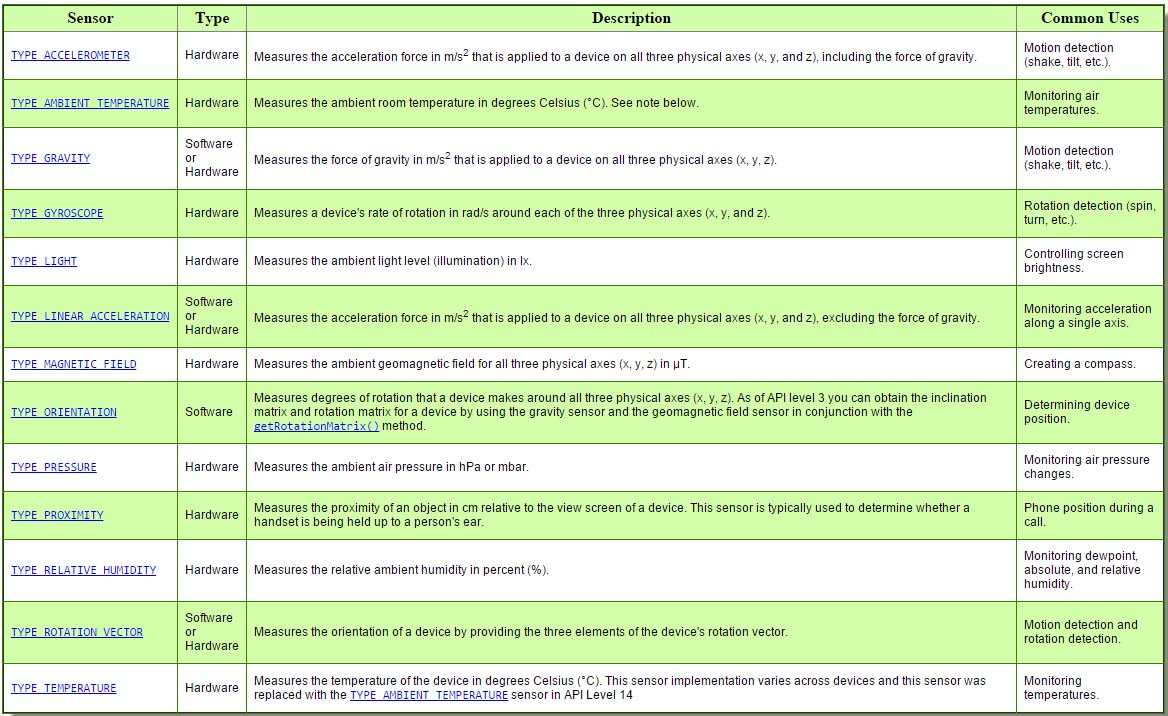
\includegraphics[width=0.99\linewidth]{figures/sensor-table}
    \end{figure}
  \end{frame}

  \begin{frame}{Sensor Management API}
    \begin{itemize}\itemsep10pt
      \item the ASF provides a series of components present in the
      \codeB{android.hardware package.*}.
      \item The most significant:
      \begin{itemize}
        \item \codeB{SensorManager}, allows you to create an instance of an
        object that represents the service associated with a specific sensor.
        Provides methods for accessing sensors and for registering listeners.
        \item \codeB{Sensor}, allows you to create specific instances for each
        supported sensor.
        \item \codeB{SensorEvent}, represents the instance for each event
        propagated by any sensor. It includes both the raw data produced by the
        sensor and the current information associated with the sensor (accuracy,
        timestamp, \dots).
        \item \codeB{SensorEventListener}, interface that must be implemented by
        any object that must be designed to receive information from sensors of
        interest. 
      \end{itemize}
  \end{itemize}

  \end{frame}

\subsection{Identification and Monitoring of Sensors}

  \begin{frame}[fragile,allowframebreaks]{Identification of available sensors}
    \begin{itemize}
      \item By accessing the \codeA{SensorManager} instance, it is possible to establish
      which sensors are currently available in the device.
      \begin{itemize}
        \item This instance can be obtained through the
        \codeB{getSystemService()} method, specifying
        \codeB{Context.SENSOR\_SERVICE} as parameter.
      \end{itemize}
    \end{itemize}

    \begin{exampleblock}{Example -- List of available sensors}
      \begin{lstlisting}[language=Java]  
private SensorManager sm;
      
@Override
protected void onCreate(Bundle savedInstanceState) {
  /* ... */
    
  sm = (SensorManager) getSystemService(Context.SENSOR_SERVICE);

  List<Sensor> sensors = sm.getSensorList(Sensor.TYPE_ALL);
}
      \end{lstlisting}
    \end{exampleblock}

    \begin{itemize}
      \item Vice versa, it is possible to check the availability of each single
      sensor using the \codeB{getDefaultSensor()} function provided by the
      \codeA{SensorManager}.
    \end{itemize}

    \begin{exampleblock}{Example -- Availability of a specific sensor}
      \begin{lstlisting}[language=Java]  
private SensorManager sm;
private Sensor accelerometer;  

@Override
protected void onCreate(Bundle savedInstanceState) {
  /* ... */
  accelerometer = sm.getDefaultSensor(Sensor.TYPE_ACCELEROMETER);
    
  if(accelerometer != null) {
    // The Accelerometer sensor is available for this device. 
  }
}
      \end{lstlisting}
    \end{exampleblock}
  \end{frame}

  \begin{frame}{Monitoring of the data produced by the sensors}
    In order to monitor the data produced by a specific sensor, it is necessary:
    \begin{enumerate}\itemsep10pt
      \item Define a specific listener by implementing the
      \codeB{SensorEventListener} interface (consisting of two specific
      callbacks):
      \begin{itemize}
        \item \codeB{onAccuracyChanged()}, invoked by the system when the
        sensor's accuracy in producing the raw data stream changes.
        \item \codeB{onSensorChanged()}, invoked by the system when new stream
        data is available to be read. The information is propagated to the
        listener through a parameter of type \codeB{SensorEvent}.
      \end{itemize}
      \item Register the listener with the \codeA{SensorManager}.
    \end{enumerate}

  \end{frame}

  \begin{frame}[fragile,allowframebreaks]{Monitoring -- Example}
    \begin{exampleblock}{Exmaple -- Ambient light sensor}
      \begin{lstlisting}[language=Java]  
public class MainActivity extends Activity {

  private SensorManager sm;
  private Sensor lightSensor;
  private LightSensorListener lsListener;

  @Override
  protected void onCreate(Bundle savedInstanceState) {
    super.onCreate(savedInstanceState);
    setContentView(/* ... */);

    sm = (SensorManager) getSystemService(Context.SENSOR_SERVICE);
    lightSensor = sm.getDefaultSensor(Sensor.TYPE_LIGHT);

    if (lightSensor != null)
      lsListener = new LightSensorListener();
  }      
      \end{lstlisting}
    \end{exampleblock}
    \begin{exampleblock}{\vspace{-10pt}}
      \begin{lstlisting}[language=Java] 
  @Override
  protected void onResume() {
    super.onResume();
    
    if(lightSensor != null)
      sm.registerListener(lsListener, lightSensor, 
            SensorManager.SENSOR_DELAY_NORMAL);
  }

  @Override
  protected void onPause() {
    super.onPause();
    
    if(lightSensor != null)
      sm.unregisterListener(lsListener);
  }
}
      \end{lstlisting}
    \end{exampleblock}

    \begin{exampleblock}{Example -- Listener definition}
      \begin{lstlisting}[language=Java]  
public class LightSensorListener implements SensorEventListener {

  private static final String LOG_TAG = "app-tag";
  
  @Override
  public void onSensorChanged(SensorEvent event) {
    float actualvalue = event.values[0];				
    Log.d(LOG_TAG,"Actual Value: " + actualvalue);
  }

  @Override
  public void onAccuracyChanged(Sensor sensor, int accuracy) {
    //do something		
  }
}
      \end{lstlisting}
    \end{exampleblock}
    \begin{itemize}\itemsep10pt
      \item The registration of the listener for a specific sensor can be done
      through the use of the \codeB{registerListener()} method provided by the
      \codeA{SensorManager}.
      \begin{itemize}
        \item The method must receive the instance of the listener and the
        sensor as input. Furthermore, the third parameter refers to the emission
        rate of the desired value.
      \end{itemize}
      \item Dually, the listener can be unregistered by calling the
      \codeB{unregisteredListener()} method.
      \item In the listener, it is possible to access the values produced by the
      specific sensor through the float vector obtainable from the \codeB{SensorEvent}
      type parameter of the \codeB{onSensorChanged()} callback.
      \begin{itemize}
        \item The number of values present in this vector varies according to
        the type of sensor being monitored.
      \end{itemize}
    \end{itemize}

  \end{frame}

  \begin{frame}{Best-practices for using sensors}
    \begin{itemize}\itemsep20pt
      \item Always unregister the listeners for the sensors in the onPause ()
      callback of the activity that uses the sensor.
      \item Do not insert blocking mechanisms into the \codeA{onSensorChanged()}
      function.
      \begin{itemize}
        \item However, the listener can use asynchronous tasks to perform
        long-running tasks on the data produced by the sensors.
      \end{itemize}
      \item Always check for the presence of sensors before using them.
    \end{itemize}
  \end{frame}

\section{Motion Sensors}

  \begin{frame}{Motion Sensors}
    \begin{itemize}\itemsep10pt
      \item The category of sensors most used and most widespread on the various
      devices is the one that refers to \underline{motion sensors}.
      \begin{itemize}
        \item \tcc{Accellerometer} and \tcc{gyroscope}, generally available as
        HW sensors, belong to this category.
      \end{itemize}
      \item The motion sensors can be used to identify the movement of the
      device with reference to the spatial coordinates.
      \item Example of application of motion sensors:
      \begin{itemize}
        \item Determine if a device is shaking.
        \item Determine the rotation of the device relative to the user.
        \item Determine if you are traveling by car or if you are walking. 
      \end{itemize}
    \end{itemize}
  \end{frame}

\subsection{Reference System}
  \begin{frame}[allowframebreaks]{Sensor Reference System}
    \begin{itemize}\itemsep10pt
      \item A three-axis (X, Y, Z) SR-based coordinate system is used.
      \item The SR is defined according to the standard orientation of the
      specific device (\textit{portrait} for most devices).
      \item When the device is in the standard position, the following applies:
      \begin{itemize}
        \item The X axis is horizontal and its positive axis is defined to the
        right
        \item The Y axis is vertical and its positive axis is identified upwards
        \item The Z axis exits the device screen orthogonally to the other two
        axes with positive direction.
      \end{itemize}
      \item Note that no swapping of the X and Y axes is done when the device is
      rotated. 
    \end{itemize}

    \begin{figure}
      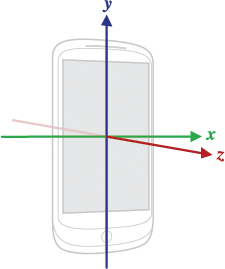
\includegraphics[width=0.5\linewidth]{figures/axis_device.png}
    \end{figure}

    \begin{itemize}\itemsep20pt
      \item The default orientation is not necessarily \textit{portrait}, many
      devices (including some tablets and all smart glasses) assume
      \textit{landscape} as the default orientation.
      \item Some sensors return their values based on the terrestrial SR rather
      than that of the device.
      \begin{itemize}
        \item It is always advisable to check this aspect before interpreting
        the values returned by a sensor and eventually applying transformation
        matrices.
      \end{itemize}
    \end{itemize}

    \link{android-developers.blogspot.it/2010/09/one-screen-turn-deserves-another.html}
  \end{frame}

\subsection{Accelerometer}

  \begin{frame}[fragile,allowframebreaks]{Accelerometer}
    \begin{itemize}
      \item Conceptually, it measures the acceleration ($m/s^{2}$) applied to
      the device along the three axes of the SR, also including the force of
      gravity.
      \begin{itemize}
        \item In a condition of equilibrium (i.e. the device is placed on a flat
        surface with the screen facing upwards) the acceleration values for the
        X and Y axes are close to zero while the acceleration value along the Z
        axis is close to the (absolute) value of the acceleration due to gravity
        9.81.
      \end{itemize}
    \end{itemize}

    \begin{exampleblock}{Example -- Accelerometer instance}
      \begin{lstlisting}[language=Java]  
SensorManager sm = ...
Sensor accelerometer = sm.getDefaultSensor(
          Sensor.TYPE_ACCELEROMETER);
      \end{lstlisting}
    \end{exampleblock}

    \begin{itemize}
      \item If you want to obtain the acceleration values without considering
      the force of gravity, you can refer to the \tcc{linear accelerometer} SW
      sensor.
    \end{itemize}

    \begin{exampleblock}{Example -- Liniear accelerometer instance}
      \begin{lstlisting}[language=Java]  
SensorManager sm = ...
Sensor linear_accelerometer = sm.getDefaultSensor(
            Sensor.TYPE_LINEAR_ACCELEROMETER);
      \end{lstlisting}
    \end{exampleblock}
    \vspace{10pt}
    \begin{itemize}
      \item In both cases, in the \codeA{onSensorChanged()} callback, it is
      possible to retrieve the acceleration \codeA{values} along X, Y and Z
      using the float vector returned by the values field of the SensorEvent
      type parameter. Specifically, the values are positioned respectively in
      the first three positions of the vector.
    \end{itemize}

  \end{frame}

\subsection{Gyroscope}

  \begin{frame}[fragile]{Giroscopio}
    \begin{itemize}\itemsep10pt
      \item Conceptually, it measures the rotation ($rad / s$) based on the three axes of the device.
      \begin{itemize}
        \item Rotation is positive in the clockwise direction.
      \end{itemize}
      \item Generally, the values obtained by the gyroscope are combined with
      the time data in order to calculate the rotation of the device considering
      the evolution of time.
    \end{itemize}

    \begin{exampleblock}{Example -- Gyroscope instance}
      \begin{lstlisting}[language=Java]  
SensorManager sm = ...
Sensor gyroscope = sm.getDefaultSensor(
          Sensor.TYPE_GYROSCOPE);
      \end{lstlisting}
    \end{exampleblock}
    \begin{itemize}
      \item Again, the values of X, Y, and Z are given as the first, second, and
      third elements of the float vector, respectively.
    \end{itemize}
  \end{frame}

\section{NFC}

  \begin{frame}{Near Field Communication (NFC)}
    \begin{itemize}\itemsep10pt
      \item NFC is a contactless short-range wireless connectivity technology.
      \begin{itemize}
        \item When two devices equipped with NFC sensors (respectively \textit{initiator}
        and \textit{target/tag}) are nearby (within 5cm), an ad-hoc P2P type network is
        created between the two for the exchange of a limited amount of data.
      \end{itemize}
      \item The reading of a generic NFC tag can be performed by interpreting
      the values of one or more NDEF (NFC Data Exchange Format) records stored
      in the tag.
      \item In Android it is possible to obtain read and write access to enabled
      NFC tags using the library implemented in the \codeB{android.nfc} package.
    \end{itemize}
  \end{frame}

  \begin{frame}[allowframebreaks]{NDEF record Structure}
    \begin{figure}
      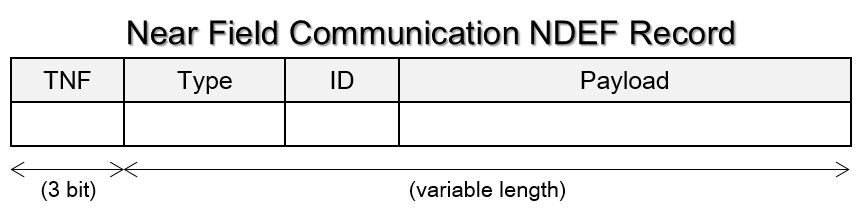
\includegraphics[width=1\linewidth]{figures/nfc_ndef_record.png}
    \end{figure}

    \begin{itemize}\itemsep20pt
      \item \tcc{TNF (Type Name Format)}, specifies how to interpret the next
      \tcc{Type} field. It can assume default values such as: \codeB{TNF\_EMPTY},
      \codeB{TNF\_ABSOLUTE\_URI}, \codeB{TNF\_EXTERNAL\_TYPE},
      \codeB{TNF\_WELL\_KNOWN},\dots.
      \item \tcc{Type}, describes the specific type assumed by the NDEF record.
      \begin{itemize}
        \item In the most common case where the \codeA{TNF\_WELL\_KNOWN} value
        has been associated with the previous TNF field, the type field must be
        used to specify a valid RDT (Record Type Description) value.
        \item In general, we tend to specify an RDT value of \codeB{RDT\_TEXT} which
        corresponds to the MIME type \codeA{text/plain}.
      \end{itemize} 
      \item \tcc{ID}, unique (optional) identifier for the record.
      \item \tcc{Paylaod}, the content of the record that will be read/write by
      the \codeA{initiator}.
    \end{itemize}
  \end{frame}

  \begin{frame}[fragile]{Permissions}
    \begin{itemize}
      \item To use the NFC support offered by the operating system, it is
      necessary to declare the intention in the File Manifest, specifying the
      following permissions.
    \end{itemize}

    \begin{exampleblock}{NFC permissions}
      \begin{lstlisting}[language=XML]
<uses-permission
    android:name="android.permission.NFC"/>
    
<uses-feature
    android:name="android.hardware.nfc" android:required="true"/>
      \end{lstlisting}
    \end{exampleblock}
    \vspace{10pt}
    {\small \textit{Note.} NFC support is available in Android starting from API
   Level 10. Therefore, to use the NFC the specified minSdkVersion must be equal
   to or greater than 10.}
  \end{frame}

\subsection{Component initialization}

  \begin{frame}[fragile,allowframebreaks]{NFC support initialization}
    \begin{itemize}\itemsep20pt
      \item In Android, the entry point for using the NFC sensor is provided by
      the \tcc{NfcAdapter} class.
      \begin{itemize}
        \item This allows you to activate the NFC sensor, identify any nearby
        tag and read or write this tag.
      \end{itemize}
      \item Access to the NFC sensor is exclusive. Each application must obtain
      and release the sensor explicitly.
      \item The identification of a tag is retro-propagated to the activity
      through an Intent, suitably filtered on the type/category.
    \end{itemize}

    \begin{exampleblock}{Example - Initialization}
      \begin{lstlisting}[language=Java]
private static final String MIME_TEXT_PLAIN = "text/plain";

private NfcAdapter nfcAdapter;

@Override
protected void onCreate(Bundle savedInstanceState){
  super.onCreate(savedInstanceState);
  setContentView(/* ... */);
    
  nfcAdapter = NfcAdapter.getDefaultAdapter(this);
  
  if(nfcAdapter == null){
    //NFC not supported
    finish();
  }
}
      \end{lstlisting}
    \end{exampleblock}

  \end{frame}

\subsection{Activation, Release and Connection}
  \begin{frame}[fragile,allowframebreaks]{Activation of NFC support}
    \begin{itemize}
      \item The activation of the NFC must be done at the same time as the
      activity enters the Running state (that is, in the \codeA{onResume()} method).
      \begin{itemize}
        \item It is based on the definition of a series of Intents that prepare
        the application in order to identify any NFC tags approaching the
        sensor.
      \end{itemize}
    \end{itemize}

    \begin{exampleblock}{Example - Start NFC Dispatching}
      \begin{lstlisting}[language=Java]
@Override
public void onResume(){
  super.onResume();
  startNFCDispatch(this, nfcAdapter);
}
      \end{lstlisting}
    \end{exampleblock}

    \begin{exampleblock}{\vspace{-10pt}}
      \begin{lstlisting}[language=Java]
private void startNFCDispatch(Activity a, NfcAdapter adapter){
  Context ctx = a.getApplicationContext();
  
  final Intent i = new Intent(ctx, a.getClass());
  i.setFlags(Intent.FLAG_ACTIVITY_SINGLE_TOP);

  final PendingIntent pi = PendingIntent.getActivity(ctx, 0, i, 0);

  IntentFilter[] filters = new IntentFilter[1];
  filters[0] = new IntentFilter();
  filters[0].addAction(NfcAdapter.ACTION_NDEF_DISCOVERED);
  filters[0].addCategory(Intent.CATEGORY_DEFAULT);
        
  try {
    filters[0].addDataType(MIME_TEXT_PLAIN);
  } catch (MalformedMimeTypeException e) { /* ... */ }
  
  String[][] techList = new String[][]{};
  adapter.enableForegroundDispatch(a, pi, filters, techList);
}
      \end{lstlisting}
    \end{exampleblock}
  \end{frame}

  \begin{frame}[fragile,allowframebreaks]{Release of NFC support}
    \begin{itemize}
      \item The release of the NFC must be done at the same time as the activity
      exits from the Running state (that is, in the \codeA{onPause()} method).
      \item Otherwise, no other application will be able to use the sensor.
    \end{itemize}
    \begin{exampleblock}{Example - Stop NFC Dispatching}
      \begin{lstlisting}[language=Java]	
@Override
protected void onPause(){
  stopNFCDispatch(this, nfcAdapter);
  super.onPause();
}

private void stopNFCDispatch(Activity a, NfcAdapter adapter){
  adapter.disableForegroundDispatch(a);
}
      \end{lstlisting}
    \end{exampleblock}
  \end{frame}

  \begin{frame}[fragile,allowframebreaks]{Connecting to an NFC tag}
    \begin{itemize}\itemsep10pt
      \item On any activity it is possible to redefine the callback
      \codeB{onNewIntent(Intent i)}.
      \begin{itemize}
        \item The system calls this method every time a PendingIntent is
        processed, suitably registered by the activity.
      \end{itemize}
      \item This is the case of NFC, since in its activation phase a specific
      PendingIntent is registered for the desired NFC tags.
      \begin{itemize}
        \item In particular, a PendingIntent has been defined which is
        associated with the NDEF type record recognition action.
      \end{itemize}
    \end{itemize}

    \begin{exampleblock}{Example - Redefinition of the \texttt{onNewIntent()} method}
      \begin{lstlisting}[language=Java]	
@Override
protected void onNewIntent(Intent intent) { 
  Tag tag = (Tag)intent.getParcelableExtra(NfcAdapter.EXTRA_TAG);
  
  if(NfcAdapter.ACTION_NDEF_DISCOVERED.equals(intent.getAction()))
    if(MIME_TEXT_PLAIN.equals(intent.getType())){
      //do something (I/O on tag)
    }
}
      \end{lstlisting}
    \end{exampleblock}
    \begin{itemize}
      \item Through the intent it is possible to retrieve an instance of the
      \codeB{Tag} type whose validity will last as long as the NFC tag is near
      the sensor.
      \item Through this instance it is possible to read or write the NFC tag.
    \end{itemize}
  \end{frame}

\subsection{NFC I/O}

  \begin{frame}[fragile,allowframebreaks]{Reading a NFC Tag}
    \begin{exampleblock}{Example - Reading the Tag's content}
      \begin{lstlisting}[language=Java]	
public String readNFCTag(Tag tag) throws Exception {
  Ndef ndef = Ndef.get(tag);

  if (ndef == null)
    return null;

  NdefRecord[] records = ndef.getCachedNdefMessage().getRecords();

  for(NdefRecord r : records)      	
    if(r.getTnf() == NdefRecord.TNF_WELL_KNOWN 
        && Arrays.equals(r.getType(), NdefRecord.RTD_TEXT))
      return analyzePayload(r.getPayload());

  return null;
}
      \end{lstlisting}
    \end{exampleblock}

    \begin{exampleblock}{\vspace{-10pt}}
      \begin{lstlisting}[language=Java]
private String analyzePayload(byte[] payload) throws Exception {
  String encoding = ((payload[0] & 0200) == 0) ? "UTF-8":"UTF-16";
  int langCodeLen = payload[0] & 0077;
  
  String tagContent = new String(payload, langCodeLen + 1,
              payload.length - langCodeLen - 1, encoding);
                              
  return tagContent;
}
      \end{lstlisting}
    \end{exampleblock}
    \begin{itemize}
      \item Each NFC tag can contain one or more NDEF records (depending on the
      size/capacity of the tag).
      \item If the NDEF record specifies the desired parameters for TNF and
      Type, it is possible to analyze the Payload to extract its content.
    \end{itemize}
  \end{frame}

  \begin{frame}[fragile,allowframebreaks]{Writing a NFC Tag}
    \begin{itemize}\itemsep10pt
      \item When writing a tag, it must remain in close proximity to the
      NFC sensor for the duration of the process 
      \item Each NDEF record created can then be written to the tag using its
      instance.
      \item The creation of the NDEF record must take place by specifying all
      the required parameters, appropriately coded.
    \end{itemize}

  \end{frame}
    
  \begin{frame}[fragile,allowframebreaks]{Reading a NFC Tag II}
    \begin{exampleblock}{Example - Writing the content of a tag}
      \begin{lstlisting}[language=Java]	
public void writeTag(String content, Tag tag) throws Exception{
  NdefRecord[] records = new NdefRecord[1];
  records[0] = createRecord(content);
  
  NdefMessage message = new NdefMessage(records);
  
  Ndef ndef = Ndef.get(tag);
  ndef.connect();
  ndef.writeNdefMessage(message);
  ndef.close();
}

private NdefRecord createRecord(String text) throws Exception {
  String lang = "en";
  byte[] textBytes = text.getBytes();
  byte[] langBytes = lang.getBytes("US-ASCII");
      \end{lstlisting}
    \end{exampleblock}
  \end{frame}

  \begin{frame}[fragile,allowframebreaks]{Reading a NFC Tag III}
    \begin{exampleblock}{\vspace{-10pt}}
      \begin{lstlisting}[language=Java]
      
  int textLength = textBytes.length;
  int langLength = langBytes.length;

  byte[] payload = new byte[1 + langLength + textLength];
  payload[0] = (byte) langLength;

  System.arraycopy(langBytes, 0, payload, 1, langLength);
  System.arraycopy(textBytes, 0, payload, 1 + langLength, textLength);
  NdefRecord recordNFC = new NdefRecord(NdefRecord.TNF_WELL_KNOWN, 
                  NdefRecord.RTD_TEXT, new byte[0], payload);
  
  return recordNFC;
}
      \end{lstlisting}
    \end{exampleblock}
  \end{frame}


\section{Geolocation in Android}
  \begin{frame}{Geolocation in Android}
    \begin{itemize}\itemsep10pt
      \item In android, access to location services, via GPS and more, is
      provided through instances of objects defined in the
      \codeB{android.location package.*}.
      \item As in the case of sensors, also for localization there is a
      \codeB{LocationManager} with which it is possible to instantiate the
      components necessary to obtain information on the user's location.
      \item Once the \codeA{LoactionManager} instance is obtained, it's
      possible: 
      \begin{itemize}
        \item Query the instance of a \codeB{LocationProvider} to know the last
        known position determined by the geolocation system.
        \item Register for periodic updates.
        \item Register Intent to be notified when the device is near specific
        locations (specified according to latitude and longitude).
      \end{itemize}
    \end{itemize}
  \end{frame}

\subsection{Network-based vs. GPS-based}
  \begin{frame}{Network-based vs. GPS-based}
    \begin{itemize}\itemsep10pt
      \item To develop location-aware applications, it is possible to use the
      GPS signal (\tcc{location GPS-Based}) and/or exploit the information that
      comes from the Internet access provider (\tcc{location Network-based})
      \item Location GPS-based:
      \begin{itemize}
        \item Very accurate information (within a few meters)
        \item It can be used almost exclusively in outdoor environments.
        \item High battery consumption.
        \item It does not provide a quick response on the user's location.
      \end{itemize}
      \item Location Network-based
      \begin{itemize}
        \item It guarantees both indoor and outdoor operation.
        \item It has a lower battery consumption.
        \item It guarantees much shorter response times.
        \item Much less precise mechanism than the previous one
      \end{itemize}
    \end{itemize}
  \end{frame}

\subsection{Informazioni sulla posizione GPS}

\subsection*{Attivare gli aggiornamenti}

  \begin{frame}[fragile,allowframebreaks]{Request location updates}
    \begin{itemize}\itemsep10pt
      \item Once the instance for the \codeB{LocationManager} has been obtained,
      it is possible to invoke the \codeB{requestLocationUpdates()} method to
      register an appropriate listener.
      \item This method accepts as parameters (in order):
      \begin{itemize}
        \item The type of location you want to use, alternatively chosen between
        \codeB{LocationManager.NETWORK\_PROVIDER} or
        \codeB{LocationManager.GPS\_PROVIDER}, 
        \item the minimum time interval, in milliseconds, that must elapse
        between one update and the next.
        \item the minimum spatial interval, in meters, between one update and the next
        \item the instance of the listener, of the \codeB{LocationListener} type.
      \end{itemize}
    \end{itemize}

    \begin{exampleblock}{Example -- Listener for location updates}
      \begin{lstlisting}[language=Java] 
LocationListener listener = new LocationListener() {
  public void onLocationChanged(Location location) {
    makeUseOfNewLocation(location);
  }

  public void onStatusChanged(String provider, int status, Bundle extras) {/* ... */}
  public void onProviderEnabled(String provider) {/* ... */}
  public void onProviderDisabled(String provider) {/* ... */}
};

LocationManager lm = (LocationManager) getSystemService(
    Context.LOCATION_SERVICE);
                                        
lm.requestLocationUpdates(LocationManager.GPS_PROVIDER, 0, 0, listener);                                        
      \end{lstlisting}
    \end{exampleblock}
  \end{frame}

\subsection*{Recall the last known position}

  \begin{frame}[fragile]{Request the last detected position}
    \begin{itemize}
      \item Often it may be necessary to know the last position detected by the
      location service without wanting to be notified every time a new position is
      detected.
      \item In this case it's possible to obtain the last known position directly
      from the \codeA{LocationManager} instance. 
    \end{itemize}

    \begin{exampleblock}{Example -- Obtain the last detected position}
      \begin{lstlisting}[language=Java]
LocationManager lm = ...

String lp = LocationManager.NETWORK_PROVIDER;
  //or LocationManager.GPS_PROVIDER

Location lastKnownLocation = lm.getLastKnownLocation(lp);
      \end{lstlisting}
    \end{exampleblock}
  \end{frame}

\subsection*{Stop the updates}

  \begin{frame}[fragile]{Stop the updates}
    \begin{itemize}\itemsep10pt
      \item Again, it is a good idea to stop the updates when the Activity
      concerned to receive them is moved to the background, or when these
      updates are no longer needed.
      \item For this purpose, the \codeB{removeUpdates()} method can be called
      on the instance of \codeA{LocationManager}. The reference to the dedicated
      listener must be passed in input to the method.
    \end{itemize}

    \begin{exampleblock}{Exemple -- Stop notifications}
      \begin{lstlisting}[language=Java]
LocationManager lm = ...
LocationListener listener = ...

lm.removeUpdates(listener);
      \end{lstlisting}
    \end{exampleblock}
  \end{frame}

\subsection{Permissions}

  \begin{frame}[fragile]{Permissions for access to location services}
    \begin{itemize}
      \item To access the localization services, you need to specify some
      permissions in the application's Manifest File.
    \end{itemize}

    \begin{exampleblock}{Example -- Permissions}
      \begin{lstlisting}[language=XML] 
<uses-permission
    android:name="android.permission.ACCESS_COARSE_LOCATION"/>
<uses-permission 
    android:name="android.permission.ACCESS_FINE_LOCATION"/>
      \end{lstlisting}
    \end{exampleblock}

    \begin{itemize}
      \item In particular, the "coarse" access allows the use of network-based
      localization while the "fine" access is used to request GPS-based
      localization.
      \item If you want to use both localizations in a combined way, it is
      sufficient to specify only the second permission (which includes the
      first).
    \end{itemize}
  \end{frame}

  \begin{frame}{Nota sui Permessi}
    \begin{itemize}
      \item From the version of Android 6.0 (API Level 23) the permissions have
      been divided into two categories (based on the features that involve the
      user's \bothquote{privacy}):
      \begin{itemize}
        \item \tcc{NORMAL}, must be requested by explicit declaration in the
        manifest file. 
        \item \tcc{DANGEROUS}, must be requested by explicit declaration in the
        manifest file and the user must explicitly accept this request. 
      \end{itemize}
    \end{itemize}
    \begin{block}{Examples of NORMAL permissions}
      \codeA{ACCESS\_NETWORK\_STATE}, \codeA{BLUETOOTH},
      \codeA{BLUETOOTH\_ADMIN}, \codeA{INTERNET}, \codeA{NFC},\dots
    \end{block}

    \begin{block}{Examples of DANGEROUS permissions}
    \codeA{CAMERA}, \codeA{ACCESS\_FINE\_LOCATION}, \codeA{ACCESS\_COARSE\_LOCATION}, \codeA{RECORD\_AUDIO}, \codeA{READ\_CONTACTS}, \codeA{READ\_EXTERNAL\_STORAGE}, \codeA{WRITE\_EXTERNAL\_STORAGE}, \dots
    \end{block}
  \end{frame}

  \begin{frame}{DANGEROUS examples}
    \begin{itemize}\itemsep10pt
      \item The system throws a \codeA{SecurityException} if you use code that
      requires a DANGEROUS permission to be executed, without having previously
      checked whether the user has explicitly granted this permission or not.
      \item In the event that the user has not granted this permission, it is
      possible to delegate its activation directly to the user.
      \begin{itemize}
        \item The system is able to notify the application about whether the
        user has granted or ignored the request to use the permission.
      \end{itemize}
    \end{itemize}
    \vfill
    \link{https://developer.android.com/training/permissions/requesting}
  \end{frame}

  \begin{frame}[fragile, allowframebreaks]{Request for DANGEROUS permissions}

    \begin{exampleblock}{Example -- \codeA{ACCESS\_FINE\_LOCATION} permission}
      \begin{lstlisting}[language=Java]
final int ACCESS_FINE_LOCATION_REQUEST = 1234;

int permission = ContextCompat.checkSelfPermission(this, 
                    Manifest.permission.ACCESS_FINE_LOCATION);

if (permission == PackageManager.PERMISSION_GRANTED){
  //OK, user has confirmed the permission
} else {
  ActivityCompat.requestPermissions(this,
      new String[] {
        Manifest.permission.ACCESS_FINE_LOCATION
      },
      ACCESS_FINE_LOCATION_REQUEST);
}
      \end{lstlisting}
    \end{exampleblock}
    \vspace{20pt}
    \begin{exampleblock}{Notification Callback}
      \begin{lstlisting}[language=Java]
@Override
public void onRequestPermissionsResult(int reqCode, String permissions[], int[] res) {

  switch (reqCode) {
    case ACCESS_FINE_LOCATION_REQUEST:
      // If request is cancelled, the result arrays are empty
      if (res.length > 0 && res[0] == PackageManager.PERMISSION_GRANTED){
        // permission was granted!
      } else {
        // permission denied!
      }
      break;
  }
}
      \end{lstlisting}
    \end{exampleblock}
  \end{frame}

\section*{Riferimenti}
%-----------------------
%--- ONLINE RESURCES ---
%-----------------------

\begin{frame}{References - Online Resources}
\begin{thebibliography}{99}
\setbeamertemplate{bibliography item}[online]

\bibitem{adAPIguide} Android Developers - Guide
\newblock \link{https://developer.android.com/guide/}

\bibitem{adAPIreference} Android Developers - API Reference
\newblock \link{https://developer.android.com/reference/}

\bibitem{adTraining} Android Developers - Samples
\newblock \link{https://developer.android.com/samples/}

\bibitem{adTraining} Android Developers - Design \& Quality
\newblock \link{https://developer.android.com/design/}

\end{thebibliography}
\end{frame}

%-----------------------
%--- BOOKS -------------
%-----------------------

%\begin{frame}{Riferimenti - Libri}
%\begin{thebibliography}{99}
%\setbeamertemplate{bibliography item}[book]
%
%\bibitem{Mednieks11} Zigurd Mednieks, Laird Dornin, G. Blake Meike, Masumi Nakamura
%\newblock \emph{Programming Android}
%\newblock O'Reilly, 2011
%
%\bibitem{Haseman13} Chris Haseman, Kevin Grant
%\newblock \emph{Beginning Android Programming: Develop and Design}
%\newblock Peachpit Press, 2013
%
%\bibitem{Schwarz13} Ronan Schwarz, Phil Dutson, James Steele, Nelson To
%\newblock \emph{The Android Developer's Cookbook : Building Applications with the Android SDK}
%\newblock Addison-Wesley, 2013 
%
%\bibitem{Neil14} Theresa Neil
%\newblock \emph{Mobile Design Pattern Gallery: UI Patterns for Smartphone App}
%\newblock O'Relly, Second Edition, 2014
%\end{thebibliography}
%\end{frame}

\end{document}